%\documentclass[crop=false]{standalone}
%\usepackage[utf8]{inputenc}
\usepackage[T1]{fontenc}
\usepackage[english]{babel}
%\usepackage[iso]{date}
\usepackage{microtype} % optional, for aesthetics
\usepackage{csquotes}
\usepackage{fontawesome}
%%%%%%%%%%%%%%%%%%%%%%%%%%%%%%%%%%%%
%			Bibliography			%
%%%%%%%%%%%%%%%%%%%%%%%%%%%%%%%%%%%%
\usepackage[backend=biber,style=numeric-comp,sorting=none,natbib=true]{biblatex}
\addbibresource{./BIB/Bibliography.bib}

%%%%%%%%%%%%%%%%%%%%%%%%%%%%%%%%%%%%
%			Hyperref				%
%%%%%%%%%%%%%%%%%%%%%%%%%%%%%%%%%%%%
\usepackage{hyperref}
\usepackage{lastpage}
\hypersetup{
	breaklinks=false,
	citecolor=red,
	colorlinks=true,
	linkcolor=red,
	menucolor=black,
	pdfauthor={Thomas Arne Hensel},
	urlcolor=blue,
	bookmarks=true
}
%%%%%%%%%%%%%%%%%%%%%%%%%%%%%%%%%%%%
%				math				%
%%%%%%%%%%%%%%%%%%%%%%%%%%%%%%%%%%%%
\usepackage{amsmath}
\usepackage{amssymb}
\usepackage{amsthm}
\usepackage{commath}
\usepackage{siunitx}
\usepackage{eulervm}
%
%%%%%%%%%%%%%%%%%%%%%%%%%%%%%%%%%%%%
%		Figures and Plotting		%
%%%%%%%%%%%%%%%%%%%%%%%%%%%%%%%%%%%%
%
%\graphicspath{{SECTIONS/GRAPHICS/}}
\usepackage[dvipsnames]{xcolor}
\usepackage{graphicx}
\usepackage{caption,subcaption}%for subfigures
\usepackage{standalone}%to separately produce standalone figures
\usepackage{import}%to import figures later
%
\usepackage{tikz}%drawings like geometries
\usetikzlibrary{calc,matrix,positioning}
\usetikzlibrary{decorations.pathmorphing,patterns}
\usepackage{tikzscale}
%
\usepackage{pgfplots}
\pgfplotsset{
    ,compat=newest%1.12
    }
\usepgfplotslibrary{groupplots}
\usepgflibrary{patterns}
\usepackage{pgfplotstable}
%%%%%%%%%%%%%%%%%%%%%%%%%%%%%%%%%%%%
%				Tables				%
%%%%%%%%%%%%%%%%%%%%%%%%%%%%%%%%%%%%
\usepackage{multirow}
\usepackage{lscape}
\usepackage{pdflscape}
\usepackage{rotating}
\usepackage{tabularx}
\usepackage{booktabs}
%%%%%%%%%%%%%%%%%%%%%%%%%%%%%%%%%%%%
%			print git-hash			%
%%%%%%%%%%%%%%%%%%%%%%%%%%%%%%%%%%%%
\usepackage{etoolbox}
\newtoggle{submissionBuild}
\settoggle{submissionBuild}{false}
\nottoggle{submissionBuild}{%
	\usepackage{gitver}
	\usepackage{soul}
	\sethlcolor{green}
}{}
%%%%%%%%%%%%%%%%%%%%%%%%%%%%%%%%%%%%
%			Headings				%
%%%%%%%%%%%%%%%%%%%%%%%%%%%%%%%%%%%%
\usepackage{fancyhdr}
\setlength{\headheight}{15pt}

\pagestyle{fancy}
%\renewcommand{\chaptermark}[1]{ \markboth{#1}{} }
%\renewcommand{\sectionmark}[1]{ \markright{#1} }

\fancyhf{}
\fancyhead[LE,RO]{\footnotesize{p. \thepage\ / \pageref{LastPage}}}
\fancyhead[RE]{\emph{ \nouppercase{\leftmark}} }
\fancyhead[LO]{\emph{ \nouppercase{\rightmark}} }
\fancyfoot[CE,CO]{\iftoggle{submissionBuild}{}{%
  	\noindent{\emph{Revision}\/}: \hl{\mbox{\#\gitVer}}
	}}


\fancypagestyle{plain}{ %
  \fancyhf{} % remove everything
  \renewcommand{\headrulewidth}{0pt} % remove lines as well
  \renewcommand{\footrulewidth}{0pt}
}
% This will set fancy headings to the top of the page. The page number will be
% accompanied by the total number of pages. That way, you will know if any page is missing.
% If you do not want this for your document, you can just use``\pagestyle{plain}``.
%
\usepackage{todonotes}
%----------------------
%       Own definitions and macros
%----------------------
%
%
%----------------------
%       Annotation
%----------------------
%
\newcommand{\blue}[1]{\textcolor{blue}{#1}}%for blue comments
%\DeclareUnicodeCharacter{FFFD}{\blue{XXXX}}%to find false displayed characters, e.g. in Bib
%%%%%%%%%%%%%%%%%%%%%%%%%%%%%%%%%%%%
%				math				%
%%%%%%%%%%%%%%%%%%%%%%%%%%%%%%%%%%%%
\tikzset{
declare function={
        f(\z,\v,\x) = \z+\v*\x-0.5*\g*\x^2;
        }
}
%Define IFO-Parameters
\newcommand{\tmin}{0.7}
\newcommand{\dtmax}{\dtstart}
\newcommand{\dtstart}{1.0}
\newcommand{\T}{2.0}
\newcommand{\zmin}{3.0}
\newcommand{\dvstart}{0.8}
\newcommand{\vstart}{1.0}
\newcommand{\zmax}{9.0}
\newcommand{\g}{0.6}
\newcommand{\keff}{1.0}
%
% Word like operators.
\DeclareMathOperator{\acosh}{arcosh}
\DeclareMathOperator{\arcosh}{arcosh}
\DeclareMathOperator{\arcsinh}{arsinh}
\DeclareMathOperator{\arsinh}{arsinh}
\DeclareMathOperator{\asinh}{arsinh}
\DeclareMathOperator{\card}{card}
\DeclareMathOperator{\csch}{cshs}
\DeclareMathOperator{\diam}{diam}
\DeclareMathOperator{\sech}{sech}
\renewcommand{\Im}{\mathop{{}\mathrm{Im}}\nolimits}
\renewcommand{\Re}{\mathop{{}\mathrm{Re}}\nolimits}

% Fourier transform.
\DeclareMathOperator{\fourier}{\ensuremath{\mathcal{F}}}

% Roman versions of “e” and “i” to serve as Euler's number and the imaginary
% constant.
\newcommand{\ee}{\eup}
\newcommand{\eup}{\mathrm e}
\newcommand{\ii}{\iup}
\newcommand{\iup}{\mathrm i}

% Symbols for the various mathematical fields (natural numbers, integers,
% rational numbers, real numbers, complex numbers).
\newcommand{\C}{\ensuremath{\mathbb C}}
\newcommand{\N}{\ensuremath{\mathbb N}}
\newcommand{\Q}{\ensuremath{\mathbb Q}}
\newcommand{\R}{\ensuremath{\mathbb R}}
\newcommand{\Z}{\ensuremath{\mathbb Z}}

% Shape like operators.
\DeclareMathOperator{\dalambert}{\Box}
\DeclareMathOperator{\laplace}{\bigtriangleup}
\newcommand{\curl}{\vnabla \times}
\newcommand{\divergence}[1]{\inner{\vnabla}{#1}}
\newcommand{\vnabla}{\vec \nabla}

\newcommand{\half}{\frac 12}

% Unit vector (German „Einheitsvektor“).
\newcommand{\ev}{\hat{\vec e}}

% Scientific notation for large numbers.
\newcommand{\e}[1]{\cdot 10^{#1}}

% Mathematician's notation for the inner (scalar, dot) product.
\newcommand{\inner}[2]{\left\langle #1, #2 \right\rangle}

% Placeholders.
\newcommand{\emesswert}{\del{\messwert \pm \messwert}}
\newcommand{\fehlt}{\textcolor{darkred}{Hier fehlen noch Inhalte.}}
\newcommand{\messwert}{\textcolor{blue}{\square}}
\newcommand{\punkte}{\textcolor{white}{xxxxx}}

% Separator for equations on a single line.
\newcommand{\eqnsep}{,\quad}

% Quantum Mechanics
\newcommand{\bra}[1]{\left\langle #1 \right|}
\newcommand{\ket}[1]{\left| #1 \right\rangle}
\newcommand{\braket}[2]{\left\langle #1 \left. \vphantom{#1 #2} \right| #2 \right\rangle}
%\begin{document}
Apart from shot noise considerations, a variety of physical phenomena constitute limiting factors for precision experiments by coupling to the velocity spread or the spatial extension of the ensemble, as is the case for the Coriolis effect, GGs, WFA or mean-field effects. In the following, we characterize different systematic and statistical effects that might limit near-future experiments beyond state of the art such as long-fountain atomic gravimeters, space-based atom interferometers and atom interferometers operated in ground-based laboratories in micro-gravity environments. Starting with intrinsic loss mechanisms due to matter-light interaction, we go on to discuss DKC as a technique to suppress sys\-te\-ma\-tic effects. An analysis of the effects of imperfect detection of the atomic sample concludes this section.
%
\subsection{Coherent manipulation}
The fidelity of the interferometric beam splitters and mirrors realized by the coherent manipulation of the atoms using light is closely connected to the phase-space properties of the atomic ensemble.

First, homogeneous excitation of the atomic ensemble requires a constant Rabi frequency over the spatial extent of the atoms, which in turn implies a laser beam size much larger than the ensemble size. 
In cases of optical power constraints, e.g. typical for space missions, the ensemble size is hence restricted in order to maintain contrast by achieving reasonable rates for coherent manipulation. 
For large free-fall times such a requirement can be translated into a maximum expansion rate of the ensemble. 
\autoref{fig:DKC_comparison} shows the significant difference in expansion rate between thermal and condensed ensembles which indicates a clear advantage of the latter especially for large interferometry time scales.
Second, for all applications outlined in the previous section, typically Doppler-sensitive two-photon couplings are employed, such that the longitudinal atomic velocity introduces a detuning. 
The temporal profile of light pulses determines their velocity acceptance and hence defines criteria for the atoms' velocity dispersion. 
In general, smaller velocity widths, corresponding to a smaller distribution of detunings, are desirable for an efficient addressing of the atoms.

An effective, simplified model~\cite{CheinetPhD} allows to assess the effects of spatial and velocity selectivity quantitatively. 
The convolution of the atoms' radial density distribution $n(\vec r,t)$  and longitudinal dispersion $f(\vec v)$ with the position- and velocity-dependent excitation rate of the pulse
\begin{equation}
    p(\vec r,\vec v,t)\propto (\Omega_0/\Omega_\text{eff})^2 \sin^2(\Omega_\text{eff} t/2)
\end{equation}
determines the total excitation rate
\begin{equation}
    \label{eq:exc-prob}
    P_\text{exc}=2\pi \int\int \vec r f(\vec v) n(\vec r,t) p(\vec r,\vec v,t) \text{d}\vec r \text{d}\vec v.
\end{equation}
Note, that the transverse velocity distribution modifies the time-dependent spatial distribution $n(\vec r,t)$. 
This treatment assumes a box pulse of duration $t$ and an effective Rabi frequency
\begin{equation}
    \Omega_\text{eff}= \sqrt{\Omega^2_0(\vec r)+(\vec k_\text{eff}\cdot\vec v)^2},
\end{equation}
where the spatial dependence of the Rabi frequency $\Omega_0(\vec r)$ is given by the radial beam profile. A similar treatment was applied in the case of a recent gravitational wave detection proposal~\cite{Loriani2019}.
%
\subsection{Wave-front aberrations}\label{sec:WFA}
Matter-light interactions in the atom interferometric cycle are typically subject to the beam's natural wave-front curvature (e.g. of a gaussian beam) and additional imperfections of the laser beam profile~\cite{Schkolnik2015,LouchetChauvet2011} caused by non-ideal optics. While errors due to the initial collimation of large beams (>2\,cm) are negligible, retro-reflection still introduces WFA that lead to a considerable systematic uncertainty. We employ a second order approximation to the deviation from flat wave-fronts for the combined effects of beam and optics.
The resulting spatial dependence of the laser phase fronts imprints a position-dependent phase on the atoms.
Depending on the amplitude and wavelength of the distortion relative to the size of the atomic ensemble, the resulting phase shift may average out, reduce contrast, lead to phase patterns that can be resolved during detection or result in an average phase shift. In state-of-the-art cold atom gravimeters, WFA induce the limiting systematic uncertainty of 30\,nm/s$^2$ to 40\,nm/s$^2$~\cite{Freier2016,Gillot2016}. A more recent analysis of the device in \cite{Gillot2016} evaluated the systematic error to 55\,nm/s$^2$ with an uncertainty of 13\,nm/s$^2$~\cite{Karcher2018}.
We limit our study case to long-scale WFA, assuming a quadratic dependency of the wave-fronts on the transverse position of the atoms, as introduced by a curvature of the retro-reflecting mirror. In this case, the resulting wave-front curvature with radius $R$ couples to the finite velocity spread $\sigma_v$ and induces the phase shift
\begin{equation}
    \label{eq:WFA}
    \sigma_{\phi_\text{WFA}}=\frac{k_\text{eff}}{R} \frac{k_B T_\text{at}}{m_\text{at}}T^2,
\end{equation}
for a Mach-Zehnder (MZ) geometry, a spatial Gaussian density distribution of the ensemble and a Gaussian velocity spread $\sigma_v$~\cite{LouchetChauvet2011}. Here, $k_\text{eff}$ denotes the effective wave vector, $T$ the interrogation time, $k_B$ is the Boltzmann constant and $T_\text{at}$, $m_\text{at}$ refer to the ensemble temperature and atomic mass, respectively.
%
\subsection{Mean-field effects}\label{subsec:MF-effects}
Mean-field effects arise due to atom-atom interactions in atomic ensembles, scale with growing densities and are an additional source for statistical errors. The mean-field energy reads
\begin{equation}
     E_\text{MF}(r)= g_\text{int}n(r)
\end{equation}
and depends on the local density $n(r)$ of the ensemble and the interaction strength $g_\text{int}^\text{BEC} = 4\pi\hbar^2a_{sc}/m_\text{at}$, where $a_{sc}$ is the s-wave scattering length. For a thermal ensemble, $g_\text{int}^\text{thermal} = 2\,g_\text{int}^\text{BEC}$~\cite{GuryOdelin2002}. Following \cite{Debs2011}, the average mean-field energy for a spherical ensemble of volume $V(t)=4\pi r(t)^3/3$ with $N_\text{at}$ atoms is consequently given by $\langle E_\text{MF}\rangle = g_\text{int} N_\text{at}/V$.
This assumes, however, a uniform density distribution with radius $r$ while thermal and BEC ensembles in fact follow a Gaussian or parabolic distribution, respectively. Hence, we take the average of the mean-field energy by weighting it with the respective density distribution:
\begin{align}
    \langle E_\text{MF}\rangle&=\frac{4 \pi \int_0^\infty dr r^2 n(r) E_\text{MF}(r)}{4 \pi \int_0^\infty dr r^2 n(r)}\notag\\
    &=g_\text{int}\frac{\int_0^\infty dr r^2 n^2(r)}{\int_0^\infty dr r^2 n(r)}\\
    \langle E_\text{MF}^\text{BEC}(t)\rangle&=\frac{15 g_\text{int}^\text{BEC} N_\text{at}^\text{BEC}}{14 \pi \sigma_r(t)^3}\\
    \langle E_\text{MF}^\text{thermal}(t)\rangle&=\frac{g_\text{int}^\text{thermal} N_\text{at}^\text{thermal}}{8 \pi^{3/2} R_\text{TF}(t)^3}
\end{align}
In case of an equal $g_\text{int}$, but unequal atomic density on the two arms of the atom interferometer, a spurious phase shift arises.
Following \cite{Debs2011}, we model the contribution by linking the imbalance in density to the initial beam splitter and neglect effects due to overlap of the two arms or losses.
If the initial beam splitter creates a superposition that deviates by $\sigma_N$ from equal probability in both states, the phase shift
\begin{equation}\label{eq:MF}
\sigma_{\phi_\text{MF}}(t) = \frac{\sigma_N}{\hbar} \int_0^t \langle E_\text{MF}(r(t'))\rangle\,\text{d}t'
\end{equation}
occurs, corresponding to the integral of the differential frequency shift between the arms.
In our assessment, we assume the initial superposition to have equal probabilities of both states on average, but to be affected by white noise with a standard deviation of $\sigma_N$ per cycle.
Without relying on quantum correlations \cite{Brif2020arxiv}, characterization of the beam splitter is limited by quantum projection noise, implying an upper limit of $\sigma_N=1/\sqrt{N_\text{at}}$ per cycle, which we adopt for our analysis.
Consequently, the mean-field-induced phase uncertainty in our model depends on the atom number and implicitly on the time-dependent ensemble size, which allows a trade-off between maximal atom number fluctuation and minimum ensemble size at the first beam splitter.
%
\subsection{Coriolis effect and gravity gradients}
Two of the most relevant systematic effects are related to the Coriolis force and GGs. The first arises due to the transverse motion of the atoms with respect to the incident beam in combination with Earth's rotation, which forms an effective Sagnac interferometer~\cite{Hogan2008,Mueller2009}. The second is the acceleration uncertainty due to the mass distribution of Earth and the apparatus surrounding the experiment. Both give rise to systematic effects as they couple to the initial kinematic conditions of the ensemble~\cite{Antoine2003}.

In the case of a MZ geometry, the uncertainty in the atom's mean velocity $\delta_v$ and mean position $\delta_r$ couple to GGs $\gamma$ parallel and perpendicular to the sensitive axis. The uncertainty in phase related to gravity gradients is given by
\begin{align}
    \label{eq:GGparallel}
    \delta_{\phi_{v,GG,{\parallel}}}&=k_\text{eff} \gamma_\parallel \delta_v T^3\\
    \delta_{\phi_{r,GG,{\parallel}}}&=k_\text{eff} \gamma_\parallel \delta_r T^2\\
    \label{eq:GGperp}
    \delta_{\phi_{v,GG,{\perp}}}&=\tfrac{14}{3} k_\text{eff} \gamma_\perp \delta_v \Omega T^4\\
    \delta_{\phi_{r,GG,{\perp}}}&=8 k_\text{eff} \gamma_\perp \delta_r \Omega T^3.
\end{align}
Due to low order of magnitude of terms related to the coupling of rotations to transverse GGs, we restrict ourselves to phase uncertainties due to gradients parallel to the sensitive axis. Residual rotations $\Omega$ perpendicular to the sensitive axis couple to the atom's velocity.
The phase uncertainty due to the Coriolis force (subscript C), is given by
\begin{equation}
    \label{eq:Rotations}
        \delta_{\phi_{v,C,{\perp}}}=2 k_\text{eff} \Omega_\perp \delta_v T^2.
\end{equation}
As the density distribution of thermal ensembles is governed by the statistics of a Gaussian density distribution, the uncertainties of the mean position $\delta_r$ and mean velocity $\delta_v$ are related to the spatial $\sigma_r$ and velocity $\sigma_v$ spread, respectively, via
\begin{equation}\label{eq:delta-sigma-relation}
    \delta_{v,r}=\sigma_{v,r}/\sqrt{N_\text{at}\nu_0}.
\end{equation}
The number of atoms $N_\text{at}$ and the number of pre-requisite measurements $\nu_0$ (i.e. the number of times the ensemble is imaged before the actual experiment) equally contribute to the statistical repetition. BECs follow a parabolic density distribution. However, this can be approximated by a Gaussian distribution via \autoref{eq:gauss-parabolic-width}, as explained in the next section.
%
\subsection{Expansion rate and collimation}
Since expansion rates have sizable effects on the precision and accuracy of atom interferometers, we discuss the possibilities offered by DKC to reduce them in this section. DKC is an established tool to further reduce the effective expansion rate of an ensemble (see~\cite{Corgier2018} and references therein). 
This phase-space-manipulation technique exploits that the free evolution of a gas released from a trap leads to a linear correlation of momentum and radial position of atoms within the ensemble. 
Recapturing the ensemble in a quadratic potential for a well-chosen duration leads to its collimation. 
Preservation of phase space density in the collisionless case requires that this reduction in momentum spread is accompanied by an increased ensemble size and hence necessitates a trade-off between desired expansion rate reduction and required growth in ensemble size. 
For non-interacting gases, i.e. thermal or fermionic gases in all regimes, this relation is captured by Liouville's theorem, 
\begin{equation}
    \sigma_{v_0}/\sigma_{v_f} =  \sigma_{r_f}/\sigma_{r_0},
\end{equation}
which states that the ratio of initial ($\sigma_{v_0}$) to final ($\sigma_{v_f}$) velocity width is inversely proportional to the relative increase in ensemble size ($\sigma_{r_f}/\sigma_{r_0}$). 
A similar relation can be found for interacting degenerate gases - for which the asymptotic final expansion rate is determined by the initial localization through Heisenberg's uncertainty principle and a mean-field contribution~\cite{Loriani2019,Castin1996,Kagan1996} - and for interacting, non-degenerate gases~\cite{GuryOdelin2002,Pedri2003}.
\autoref{fig:DKC_comparison} illustrates a DKC sequence collimating a BEC and a thermal ensemble with typical parameters.
%
\begin{figure}[h!]
    \centering
    %\documentclass{standalone}
%\usepackage[utf8]{inputenc}
\usepackage[T1]{fontenc}
\usepackage[english]{babel}
%\usepackage[iso]{date}
\usepackage{microtype} % optional, for aesthetics
\usepackage{csquotes}
\usepackage{fontawesome}
%%%%%%%%%%%%%%%%%%%%%%%%%%%%%%%%%%%%
%			Bibliography			%
%%%%%%%%%%%%%%%%%%%%%%%%%%%%%%%%%%%%
\usepackage[backend=biber,style=numeric-comp,sorting=none,natbib=true]{biblatex}
\addbibresource{./BIB/Bibliography.bib}

%%%%%%%%%%%%%%%%%%%%%%%%%%%%%%%%%%%%
%			Hyperref				%
%%%%%%%%%%%%%%%%%%%%%%%%%%%%%%%%%%%%
\usepackage{hyperref}
\usepackage{lastpage}
\hypersetup{
	breaklinks=false,
	citecolor=red,
	colorlinks=true,
	linkcolor=red,
	menucolor=black,
	pdfauthor={Thomas Arne Hensel},
	urlcolor=blue,
	bookmarks=true
}
%%%%%%%%%%%%%%%%%%%%%%%%%%%%%%%%%%%%
%				math				%
%%%%%%%%%%%%%%%%%%%%%%%%%%%%%%%%%%%%
\usepackage{amsmath}
\usepackage{amssymb}
\usepackage{amsthm}
\usepackage{commath}
\usepackage{siunitx}
\usepackage{eulervm}
%
%%%%%%%%%%%%%%%%%%%%%%%%%%%%%%%%%%%%
%		Figures and Plotting		%
%%%%%%%%%%%%%%%%%%%%%%%%%%%%%%%%%%%%
%
%\graphicspath{{SECTIONS/GRAPHICS/}}
\usepackage[dvipsnames]{xcolor}
\usepackage{graphicx}
\usepackage{caption,subcaption}%for subfigures
\usepackage{standalone}%to separately produce standalone figures
\usepackage{import}%to import figures later
%
\usepackage{tikz}%drawings like geometries
\usetikzlibrary{calc,matrix,positioning}
\usetikzlibrary{decorations.pathmorphing,patterns}
\usepackage{tikzscale}
%
\usepackage{pgfplots}
\pgfplotsset{
    ,compat=newest%1.12
    }
\usepgfplotslibrary{groupplots}
\usepgflibrary{patterns}
\usepackage{pgfplotstable}
%%%%%%%%%%%%%%%%%%%%%%%%%%%%%%%%%%%%
%				Tables				%
%%%%%%%%%%%%%%%%%%%%%%%%%%%%%%%%%%%%
\usepackage{multirow}
\usepackage{lscape}
\usepackage{pdflscape}
\usepackage{rotating}
\usepackage{tabularx}
\usepackage{booktabs}
%%%%%%%%%%%%%%%%%%%%%%%%%%%%%%%%%%%%
%			print git-hash			%
%%%%%%%%%%%%%%%%%%%%%%%%%%%%%%%%%%%%
\usepackage{etoolbox}
\newtoggle{submissionBuild}
\settoggle{submissionBuild}{false}
\nottoggle{submissionBuild}{%
	\usepackage{gitver}
	\usepackage{soul}
	\sethlcolor{green}
}{}
%%%%%%%%%%%%%%%%%%%%%%%%%%%%%%%%%%%%
%			Headings				%
%%%%%%%%%%%%%%%%%%%%%%%%%%%%%%%%%%%%
\usepackage{fancyhdr}
\setlength{\headheight}{15pt}

\pagestyle{fancy}
%\renewcommand{\chaptermark}[1]{ \markboth{#1}{} }
%\renewcommand{\sectionmark}[1]{ \markright{#1} }

\fancyhf{}
\fancyhead[LE,RO]{\footnotesize{p. \thepage\ / \pageref{LastPage}}}
\fancyhead[RE]{\emph{ \nouppercase{\leftmark}} }
\fancyhead[LO]{\emph{ \nouppercase{\rightmark}} }
\fancyfoot[CE,CO]{\iftoggle{submissionBuild}{}{%
  	\noindent{\emph{Revision}\/}: \hl{\mbox{\#\gitVer}}
	}}


\fancypagestyle{plain}{ %
  \fancyhf{} % remove everything
  \renewcommand{\headrulewidth}{0pt} % remove lines as well
  \renewcommand{\footrulewidth}{0pt}
}
% This will set fancy headings to the top of the page. The page number will be
% accompanied by the total number of pages. That way, you will know if any page is missing.
% If you do not want this for your document, you can just use``\pagestyle{plain}``.
%
\usepackage{todonotes}
%----------------------
%       Own definitions and macros
%----------------------
%
%
%----------------------
%       Annotation
%----------------------
%
\newcommand{\blue}[1]{\textcolor{blue}{#1}}%for blue comments
%\DeclareUnicodeCharacter{FFFD}{\blue{XXXX}}%to find false displayed characters, e.g. in Bib
%%%%%%%%%%%%%%%%%%%%%%%%%%%%%%%%%%%%
%				math				%
%%%%%%%%%%%%%%%%%%%%%%%%%%%%%%%%%%%%
\tikzset{
declare function={
        f(\z,\v,\x) = \z+\v*\x-0.5*\g*\x^2;
        }
}
%Define IFO-Parameters
\newcommand{\tmin}{0.7}
\newcommand{\dtmax}{\dtstart}
\newcommand{\dtstart}{1.0}
\newcommand{\T}{2.0}
\newcommand{\zmin}{3.0}
\newcommand{\dvstart}{0.8}
\newcommand{\vstart}{1.0}
\newcommand{\zmax}{9.0}
\newcommand{\g}{0.6}
\newcommand{\keff}{1.0}
%
% Word like operators.
\DeclareMathOperator{\acosh}{arcosh}
\DeclareMathOperator{\arcosh}{arcosh}
\DeclareMathOperator{\arcsinh}{arsinh}
\DeclareMathOperator{\arsinh}{arsinh}
\DeclareMathOperator{\asinh}{arsinh}
\DeclareMathOperator{\card}{card}
\DeclareMathOperator{\csch}{cshs}
\DeclareMathOperator{\diam}{diam}
\DeclareMathOperator{\sech}{sech}
\renewcommand{\Im}{\mathop{{}\mathrm{Im}}\nolimits}
\renewcommand{\Re}{\mathop{{}\mathrm{Re}}\nolimits}

% Fourier transform.
\DeclareMathOperator{\fourier}{\ensuremath{\mathcal{F}}}

% Roman versions of “e” and “i” to serve as Euler's number and the imaginary
% constant.
\newcommand{\ee}{\eup}
\newcommand{\eup}{\mathrm e}
\newcommand{\ii}{\iup}
\newcommand{\iup}{\mathrm i}

% Symbols for the various mathematical fields (natural numbers, integers,
% rational numbers, real numbers, complex numbers).
\newcommand{\C}{\ensuremath{\mathbb C}}
\newcommand{\N}{\ensuremath{\mathbb N}}
\newcommand{\Q}{\ensuremath{\mathbb Q}}
\newcommand{\R}{\ensuremath{\mathbb R}}
\newcommand{\Z}{\ensuremath{\mathbb Z}}

% Shape like operators.
\DeclareMathOperator{\dalambert}{\Box}
\DeclareMathOperator{\laplace}{\bigtriangleup}
\newcommand{\curl}{\vnabla \times}
\newcommand{\divergence}[1]{\inner{\vnabla}{#1}}
\newcommand{\vnabla}{\vec \nabla}

\newcommand{\half}{\frac 12}

% Unit vector (German „Einheitsvektor“).
\newcommand{\ev}{\hat{\vec e}}

% Scientific notation for large numbers.
\newcommand{\e}[1]{\cdot 10^{#1}}

% Mathematician's notation for the inner (scalar, dot) product.
\newcommand{\inner}[2]{\left\langle #1, #2 \right\rangle}

% Placeholders.
\newcommand{\emesswert}{\del{\messwert \pm \messwert}}
\newcommand{\fehlt}{\textcolor{darkred}{Hier fehlen noch Inhalte.}}
\newcommand{\messwert}{\textcolor{blue}{\square}}
\newcommand{\punkte}{\textcolor{white}{xxxxx}}

% Separator for equations on a single line.
\newcommand{\eqnsep}{,\quad}

% Quantum Mechanics
\newcommand{\bra}[1]{\left\langle #1 \right|}
\newcommand{\ket}[1]{\left| #1 \right\rangle}
\newcommand{\braket}[2]{\left\langle #1 \left. \vphantom{#1 #2} \right| #2 \right\rangle}
%\begin{document}
%
%----------------------
%       Data Import
%----------------------
%
\newcommand{\dataBECdkc}{../xy/dkc_BEC.dat}
\newcommand{\dataBECnodkc}{../xy/nodkc_BEC.dat}
\newcommand{\dataCLSdkc}{../xy/dkc_CLS.dat}
\newcommand{\dataCLSnodkc}{../xy/nodkc_CLS.dat}

\begin{tikzpicture}
\begin{groupplot}[
	group style={
	    group size= 2 by 1, 
	    horizontal sep = 0.4cm,
	    xticklabels at=edge bottom
},
	%width=1/2*\linewidth+0.1cm,
    %height=1.2*(1/2*\linewidth+0.1cm),
    legend style={nodes={scale=0.8, transform shape}}
]

%Small times ============================
\nextgroupplot[
	xmin=0, xmax=0.55,
	ymin=0, ymax=3.1,	
	ylabel={$2\,\sigma_r(t)$\,(mm)},
	restrict y to domain=0:3.1,
	axis y line*= left,
	xtick={0,0.25,0.5,0.55},
	xticklabels={0,0.25,0.5,}
]

%data curves
\addplot +[blue,thick,mark=none] table[x index=0, y index=1] {\dataBECdkc};
\addplot +[blue,thick,dashed,mark=none, forget plot] table[x index=0, y index=1] {\dataBECnodkc};
\addplot +[red,thick,mark=none] table[x index=0, y index=1] {\dataCLSdkc};
\addplot +[red,thick,dashed,mark=none, forget plot] table[x index=0, y index=1] {\dataCLSnodkc};

%dashed vertical line
\draw[dotted, thin] ({axis cs:0.025,0}|-{rel axis cs:0,1}) -- ({axis cs:0.025,0}|-{rel axis cs:0,0});

%coordinates for discontinuity
\coordinate (c11) at (rel axis cs:0,1);
\coordinate (c12) at (rel axis cs:1,1);
\coordinate (c21) at (rel axis cs:0,0);
\coordinate (c22) at (rel axis cs:1,0);

%Large times ============================
\nextgroupplot[
	xmin=1, xmax=10.1,
	ymin=0, ymax=82,	
	restrict y to domain=0:80,
	axis y line*=right,
	xtick={1,2,4,6,8,10},
	xticklabels={,2,4,6,8,10},
	ytick={0,20,40,60,80},
	yticklabels={0,20,40,60,80}
]

%data curves
\addplot +[blue,thick,mark=none,restrict x to domain=1:10] table[x index=0, y index=1] {\dataBECdkc};
\addplot +[blue,thick,dashed,mark=none, forget plot,restrict x to domain=1:10] table[x index=0, y index=1] {\dataBECnodkc};
\addplot +[red,thick,mark=none,restrict x to domain=1:10] table[x index=0, y index=1] {\dataCLSdkc};
\addplot +[red,thick,dashed,mark=none, forget plot,restrict x to domain=1:10] table[x index=0, y index=1] {\dataCLSnodkc};

%legend
\addlegendentry{$^{87}$Rb BEC};
\addlegendentry{$^{87}$Rb thermal};

%coordinates for discontinuity
\coordinate (c13) at (rel axis cs:0,1);
\coordinate (c14) at (rel axis cs:1,1);
\coordinate (c23) at (rel axis cs:0,0);
\coordinate (c24) at (rel axis cs:1,0);

\end{groupplot}

%common x-axis label
\node[black] at ( $ (c21)!1/2!(c24) +(0,-0.75)$ |-0,-5.5) {t (s)};

%hacked discontinuity
\filldraw[color=gray,opacity=0.2] (c12)--(c13)--(c23)--(c22);
\draw[black, dotted,thick] (c12)--(c13);
\draw[black, dotted,thick] (c22)--(c23);

\end{tikzpicture}
%\end{document}
    %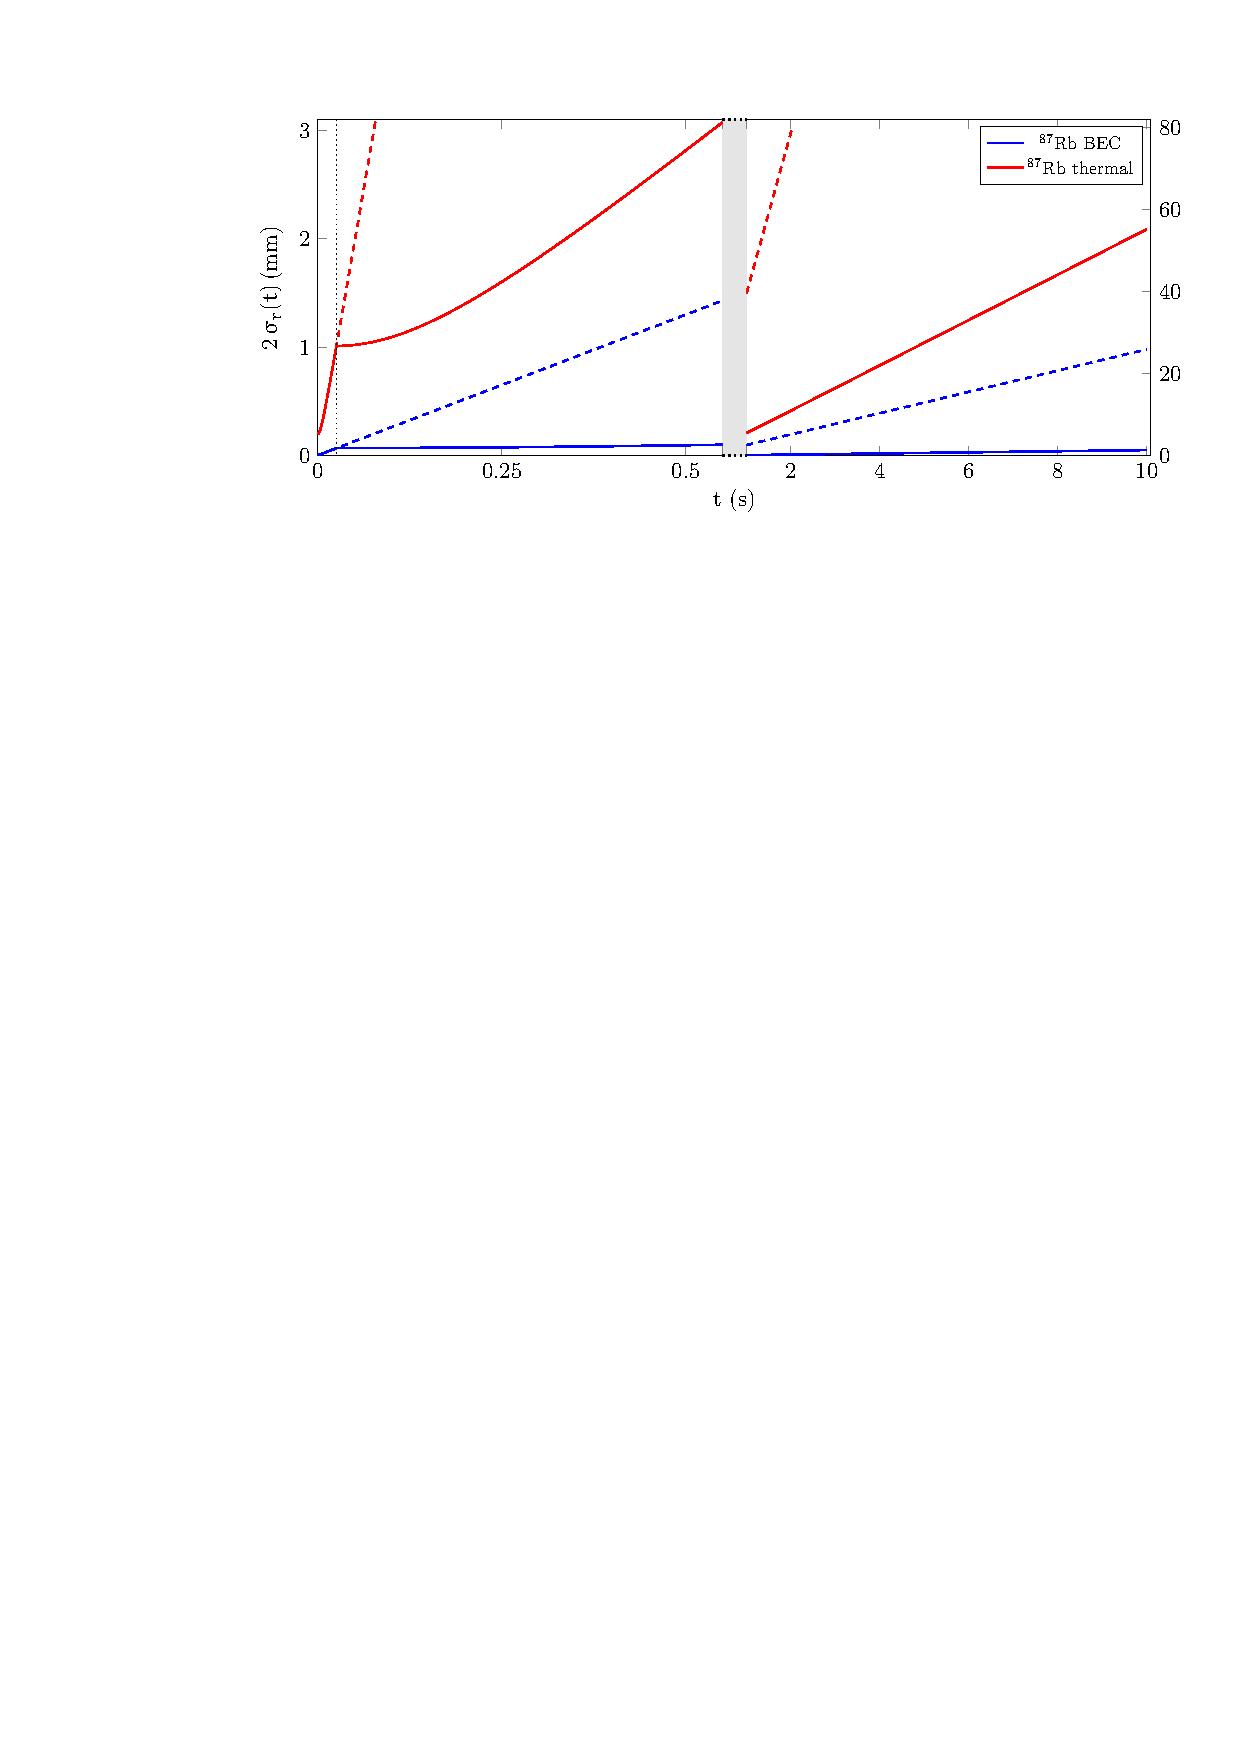
\includegraphics[width=\linewidth]{../DKC-plot-dual}
    \caption{Size evolution of thermal ensembles (red) and BECs (blue) after release from a trap. A DKC stage is reducing the expansion energies down to 80\,nK and 50\,pK for the thermal and BEC ensembles, respectively (see \autoref{tab:DKC} for the exact parameters). The dashed lines illustrate the expansion in the freely expanding case without collimation. 
    }
   \label{fig:DKC_comparison}
\end{figure}
%
The free expansion of the thermal ensemble is governed by the expansion law
\begin{equation}
    \label{eq:expansion-law}
    \sigma_r (t)=\sqrt{\sigma_{r_0}^2+\sigma_{v_f}^2t^2},
\end{equation}
whereas the BEC dynamics are captured by corresponding scaling laws~\cite{Castin1996}. As an exemplary case, we take a thermal ensemble of $10^9$ $^{87}$Rb atoms at 2\,$\mu$K with a diameter of $2\sigma_r=0.2$\,mm and collimate it down to 80\,nK, such that the required size at lens is $2 \sigma_r(t_\text{DKC})=1$\,mm. For a BEC, we assume an ensemble of $10^6$ $^{87}$Rb atoms and collimate it to 50\,pK in a trap with frequencies of $50\times 2\pi$\,Hz. These are regime-typical parameters for experiments with either thermal ensembles or BECs~\cite{Loriani2019,Mntinga2013,Kovachy2015}. Following~\cite{Loriani2019}, the expansion energies for the thermal atoms and the chemical potential $\mu_\text{BEC}$ of the BEC are obtained from
\begin{align}
    E_\text{thermal}(0)&=\tfrac{3}{2}k_B T_\text{at}(0)\\
    \mu_\text{BEC}(0)&=\tfrac{1}{2} m \omega^2 R_\text{TF}(0)^2\\
    E_\text{thermal}(t_\text{DKC})&=\tfrac{3}{2} k_B T_\text{at}(t_\text{DKC})\\
    E_\text{BEC}(t_\text{DKC})&=\tfrac{1}{2}m\left(\sigma_v(t_\text{DKC})/\sqrt{7}\right)^2
\end{align}
For a better comparison of the two fundamentally dif\-fe\-rent density distributions, the Thomas-Fermi radius $R_\text{TF}$ of the isotropic BEC with parabolic density distribution can be related to a Gaussian spatial width $\sigma_r$ via~\cite{Corgier2018} 
\begin{equation}\label{eq:gauss-parabolic-width}
    R_\text{TF}(t)=\sigma_r(t)\sqrt{7}.
\end{equation}
The resulting characteristics of the collimation sequence for $^{87}$Rb and $^{41}$K ensembles are given in \autoref{tab:DKC}.
%
\begin{center}
    \begin{table}[h!]
    \caption{Parameters of the DKC sequence of $^{87}$Rb and $^{41}$K in the thermal and condensed regime.}
    \centering
    %\subimport{GRAPHICS/}{table-DKC-parameters.tex}
    %\documentclass{standalone}
%\usepackage[utf8]{inputenc}
\usepackage[T1]{fontenc}
\usepackage[english]{babel}
%\usepackage[iso]{date}
\usepackage{microtype} % optional, for aesthetics
\usepackage{csquotes}
\usepackage{fontawesome}
%%%%%%%%%%%%%%%%%%%%%%%%%%%%%%%%%%%%
%			Bibliography			%
%%%%%%%%%%%%%%%%%%%%%%%%%%%%%%%%%%%%
\usepackage[backend=biber,style=numeric-comp,sorting=none,natbib=true]{biblatex}
\addbibresource{./BIB/Bibliography.bib}

%%%%%%%%%%%%%%%%%%%%%%%%%%%%%%%%%%%%
%			Hyperref				%
%%%%%%%%%%%%%%%%%%%%%%%%%%%%%%%%%%%%
\usepackage{hyperref}
\usepackage{lastpage}
\hypersetup{
	breaklinks=false,
	citecolor=red,
	colorlinks=true,
	linkcolor=red,
	menucolor=black,
	pdfauthor={Thomas Arne Hensel},
	urlcolor=blue,
	bookmarks=true
}
%%%%%%%%%%%%%%%%%%%%%%%%%%%%%%%%%%%%
%				math				%
%%%%%%%%%%%%%%%%%%%%%%%%%%%%%%%%%%%%
\usepackage{amsmath}
\usepackage{amssymb}
\usepackage{amsthm}
\usepackage{commath}
\usepackage{siunitx}
\usepackage{eulervm}
%
%%%%%%%%%%%%%%%%%%%%%%%%%%%%%%%%%%%%
%		Figures and Plotting		%
%%%%%%%%%%%%%%%%%%%%%%%%%%%%%%%%%%%%
%
%\graphicspath{{SECTIONS/GRAPHICS/}}
\usepackage[dvipsnames]{xcolor}
\usepackage{graphicx}
\usepackage{caption,subcaption}%for subfigures
\usepackage{standalone}%to separately produce standalone figures
\usepackage{import}%to import figures later
%
\usepackage{tikz}%drawings like geometries
\usetikzlibrary{calc,matrix,positioning}
\usetikzlibrary{decorations.pathmorphing,patterns}
\usepackage{tikzscale}
%
\usepackage{pgfplots}
\pgfplotsset{
    ,compat=newest%1.12
    }
\usepgfplotslibrary{groupplots}
\usepgflibrary{patterns}
\usepackage{pgfplotstable}
%%%%%%%%%%%%%%%%%%%%%%%%%%%%%%%%%%%%
%				Tables				%
%%%%%%%%%%%%%%%%%%%%%%%%%%%%%%%%%%%%
\usepackage{multirow}
\usepackage{lscape}
\usepackage{pdflscape}
\usepackage{rotating}
\usepackage{tabularx}
\usepackage{booktabs}
%%%%%%%%%%%%%%%%%%%%%%%%%%%%%%%%%%%%
%			print git-hash			%
%%%%%%%%%%%%%%%%%%%%%%%%%%%%%%%%%%%%
\usepackage{etoolbox}
\newtoggle{submissionBuild}
\settoggle{submissionBuild}{false}
\nottoggle{submissionBuild}{%
	\usepackage{gitver}
	\usepackage{soul}
	\sethlcolor{green}
}{}
%%%%%%%%%%%%%%%%%%%%%%%%%%%%%%%%%%%%
%			Headings				%
%%%%%%%%%%%%%%%%%%%%%%%%%%%%%%%%%%%%
\usepackage{fancyhdr}
\setlength{\headheight}{15pt}

\pagestyle{fancy}
%\renewcommand{\chaptermark}[1]{ \markboth{#1}{} }
%\renewcommand{\sectionmark}[1]{ \markright{#1} }

\fancyhf{}
\fancyhead[LE,RO]{\footnotesize{p. \thepage\ / \pageref{LastPage}}}
\fancyhead[RE]{\emph{ \nouppercase{\leftmark}} }
\fancyhead[LO]{\emph{ \nouppercase{\rightmark}} }
\fancyfoot[CE,CO]{\iftoggle{submissionBuild}{}{%
  	\noindent{\emph{Revision}\/}: \hl{\mbox{\#\gitVer}}
	}}


\fancypagestyle{plain}{ %
  \fancyhf{} % remove everything
  \renewcommand{\headrulewidth}{0pt} % remove lines as well
  \renewcommand{\footrulewidth}{0pt}
}
% This will set fancy headings to the top of the page. The page number will be
% accompanied by the total number of pages. That way, you will know if any page is missing.
% If you do not want this for your document, you can just use``\pagestyle{plain}``.
%
\usepackage{todonotes}
%----------------------
%       Own definitions and macros
%----------------------
%
%
%----------------------
%       Annotation
%----------------------
%
\newcommand{\blue}[1]{\textcolor{blue}{#1}}%for blue comments
%\DeclareUnicodeCharacter{FFFD}{\blue{XXXX}}%to find false displayed characters, e.g. in Bib
%%%%%%%%%%%%%%%%%%%%%%%%%%%%%%%%%%%%
%				math				%
%%%%%%%%%%%%%%%%%%%%%%%%%%%%%%%%%%%%
\tikzset{
declare function={
        f(\z,\v,\x) = \z+\v*\x-0.5*\g*\x^2;
        }
}
%Define IFO-Parameters
\newcommand{\tmin}{0.7}
\newcommand{\dtmax}{\dtstart}
\newcommand{\dtstart}{1.0}
\newcommand{\T}{2.0}
\newcommand{\zmin}{3.0}
\newcommand{\dvstart}{0.8}
\newcommand{\vstart}{1.0}
\newcommand{\zmax}{9.0}
\newcommand{\g}{0.6}
\newcommand{\keff}{1.0}
%
% Word like operators.
\DeclareMathOperator{\acosh}{arcosh}
\DeclareMathOperator{\arcosh}{arcosh}
\DeclareMathOperator{\arcsinh}{arsinh}
\DeclareMathOperator{\arsinh}{arsinh}
\DeclareMathOperator{\asinh}{arsinh}
\DeclareMathOperator{\card}{card}
\DeclareMathOperator{\csch}{cshs}
\DeclareMathOperator{\diam}{diam}
\DeclareMathOperator{\sech}{sech}
\renewcommand{\Im}{\mathop{{}\mathrm{Im}}\nolimits}
\renewcommand{\Re}{\mathop{{}\mathrm{Re}}\nolimits}

% Fourier transform.
\DeclareMathOperator{\fourier}{\ensuremath{\mathcal{F}}}

% Roman versions of “e” and “i” to serve as Euler's number and the imaginary
% constant.
\newcommand{\ee}{\eup}
\newcommand{\eup}{\mathrm e}
\newcommand{\ii}{\iup}
\newcommand{\iup}{\mathrm i}

% Symbols for the various mathematical fields (natural numbers, integers,
% rational numbers, real numbers, complex numbers).
\newcommand{\C}{\ensuremath{\mathbb C}}
\newcommand{\N}{\ensuremath{\mathbb N}}
\newcommand{\Q}{\ensuremath{\mathbb Q}}
\newcommand{\R}{\ensuremath{\mathbb R}}
\newcommand{\Z}{\ensuremath{\mathbb Z}}

% Shape like operators.
\DeclareMathOperator{\dalambert}{\Box}
\DeclareMathOperator{\laplace}{\bigtriangleup}
\newcommand{\curl}{\vnabla \times}
\newcommand{\divergence}[1]{\inner{\vnabla}{#1}}
\newcommand{\vnabla}{\vec \nabla}

\newcommand{\half}{\frac 12}

% Unit vector (German „Einheitsvektor“).
\newcommand{\ev}{\hat{\vec e}}

% Scientific notation for large numbers.
\newcommand{\e}[1]{\cdot 10^{#1}}

% Mathematician's notation for the inner (scalar, dot) product.
\newcommand{\inner}[2]{\left\langle #1, #2 \right\rangle}

% Placeholders.
\newcommand{\emesswert}{\del{\messwert \pm \messwert}}
\newcommand{\fehlt}{\textcolor{darkred}{Hier fehlen noch Inhalte.}}
\newcommand{\messwert}{\textcolor{blue}{\square}}
\newcommand{\punkte}{\textcolor{white}{xxxxx}}

% Separator for equations on a single line.
\newcommand{\eqnsep}{,\quad}

% Quantum Mechanics
\newcommand{\bra}[1]{\left\langle #1 \right|}
\newcommand{\ket}[1]{\left| #1 \right\rangle}
\newcommand{\braket}[2]{\left\langle #1 \left. \vphantom{#1 #2} \right| #2 \right\rangle}
%\begin{document}
%
\begin{tabular}{@{}l|ll|ll@{}}
\toprule
\multicolumn{1}{c|}{\multirow{2}{*}{Parameter\textbackslash{}Species}} & $^{87}$Rb     & $^{41}$K     & $^{87}$Rb              & $^{41}$K               \\
\multicolumn{1}{c|}{}                                                  & \multicolumn{2}{c|}{thermal} & \multicolumn{2}{c}{BEC}                         \\ \midrule
T$_\text{at}(0)$ / $\mu(0)$ ($\mu$K)                                   & \multicolumn{2}{c|}{2}       & 0.092                  & 0.064                  \\
T$_\text{at}(t_\text{DKC})$ / $\mu(t_\text{DKC})$ (nK)                 & \multicolumn{2}{c|}{80}      & \multicolumn{2}{c}{0.025}                       \\
t$_\text{DKC}$ (ms)                                                    & \multicolumn{2}{c|}{25}      & \multicolumn{1}{c}{26} & \multicolumn{1}{c}{23} \\ \midrule
2$\sigma_r(0)$ (mm)                                                    & 0.2           & 0.3          & 0.010                  & 0.013                  \\
2$\sigma_r(t_\text{DKC})$ (mm)                                         & 1.0           & 1.5          & 0.071                  & 0.079                  \\
$\sigma_v(0)$ (mm/s)                                                   & 14            & 20           & 11                     & 14                     \\
$\sigma_v(t_\text{DKC})$ (mm/s)                                        & 2.770         & 4.130        & 0.183                  & 0.273                  \\
2$\sigma_r(t_\text{DKC}+0.15\,s)$ (mm)                                 & 1.3           & 2.0          & 0.074                  & 0.084                  \\
2$\sigma_r(t_\text{DKC}+0.5\,s)$ (mm)                                  & 3.0           & 4.4          & 0.099                  & 0.130                  \\
2$\sigma_r(t_\text{DKC}+10\,s)$ (mm)                                   & 55            & 83           & 1.385                  & 2.067                  \\ \bottomrule
\end{tabular}
%
%\end{document}
    \label{tab:DKC}
    \end{table}
\end{center}
%
The illustrated collimation sequence assumes similar free expansion time $t_\text{DKC}$ prior to application of the lens for both regimes. In order to achieve a final expansion behaviour of the thermal ensemble similar to the BEC case, $t_\text{DKC}$ would need to be significantly increased (about two orders of magnitude, depending on the initial temperature), corresponding to a substantially larger ensemble size at the time of the lens~\cite{Loriani2019}.
This is a distinct disadvantage for thermal ensembles, since the DKC technique crucially depends on the harmonicity of the applied lens potential, which has to be verified over the entire spatial extent of the ensemble~\cite{Rudolph2015}.
Application of velocity-selective pulses for temperature reduction in 1D has the disadvantage of atom loss \cite{Kasevich1991}. It is therefore not a promising pathway to reach expansion rates for thermal ensembles comparable to those of BECs. Raman sideband cooling \cite{Hamann1998,Vuleti1998,Estey2015} might be a better alternative for thermal ensembles even if it is limited to about an order of magnitude larger temperatures than what the BEC ensembles could reach.
%
\subsection{Contrast and detection}
Output states of atom interferometers can be detected by absorption or fluorescence imaging methods.
Which method is appropriate depends on the experimental parameters and the information one wants to acquire.
One main distinction is whether the relative atom numbers in the output port are counted or if atomic density distributions have to be spatially resolved.
Atom number counting is commonly done with fluorescence imaging of the ensembles at the output ports, which relies on the excitation and successive emission of photons by the atoms that are then detected by a simple photo diode or CCD ca\-me\-ra.
The ensemble has to be excited by a laser beam, which means that it has to have a reasonably compact size to be illuminated.
This can usually be achieved with thermal ensembles as well as BECs.
The number of atoms contributing constructively to the signal at the output port is given by the product of the excitation probabilities at all interaction times $t_i$:
\begin{equation}
    \label{eq:contrast}
    C(t_n)=p(t_n)=\prod\limits_{i = 0}^{n}\text{P}_\text{exc}(t_i).
\end{equation}
The contrast C is given by \autoref{eq:contrast} as the convoluted excitation probability for a given phase-space distribution of the ensemble. Inhomogeneous excitation efficiency or phase gradients e.g. caused by GGs may wash out the contrast~\cite{Aguilera2014}.

In experiments employing spatial mapping of the output port wave function for the determination of the phase or analysis of features within the atomic ensemble~\cite{Sugarbaker2013}, good spatial resolution along with a high signal-to-noise ratio and minimal systematic effects during detection are required.
BECs with small spatial spread and expansion rates are thus favored over thermal ensembles to increase the spatial resolution of the CCD picture.
Indeed, the high expansion rates of thermal ensembles may at long times lead to densities challenging for absorption imaging due to decreasing signal per volume.
%\end{document}